\subsection{Team Management}
  \subsubsection{Team Collaboration}

    Through the use of frequent stand up meetings combined with daily group programming sessions and online communication, we established a very effective group development environment. We have detailed the main points below:

    %I'm avoiding the use of the title 'pair programming' here since that's not what we did or this sentance implies
    \paragraph{Coding Sessions} We often developed alongside at least one other member of the group, using a specific area in the labs to work on the project which became a hub for development. We employed a collaborative approach to development by continuously communicating with each other for advice or alternative implementations. This significantly enhanced development since each member had specific roles and knowledge areas and thus could help other people out when their work areas overlapped. As a group we did, however, maintain an overall understanding of the system and its progress and so could collaboratively help each other.

    \paragraph{Stand ups} Every day we would try to have a team stand up. Stand ups are really good for keeping on track of a project since they:
    \begin{itemize}
        \item Require mandatory participation: everyone attends and so they are always aware of how the project is moving on.
        \item Have a set structure: `What did I accomplish yesterday?', `What will I do today?', `What obstacles are impeding my progress?'.
        \item Are snappy and efficient: Due to their short nature, points are put across clearly.
    \end{itemize}
    These turned out to be one of our best collaboration methods, and after stand ups any group decisions that needed to be made could be made. There was never any repetition or people missing out on something because they hadn't been told.
    Whilst away for the Christmas holidays we tried to maintain these stand ups through Skype\cite{skype} calls in order for us to continuously update the group on what we'd been working on. However since it was the holidays these were a little more infrequent.

    \paragraph{Trello\cite{trello}} is an online project management application which uses boards containing lists of tasks that need to be completed. Each list is made up of cards which are themselves interactive and can contain checkboxes, comments, due dates etc. We used Trello at the start of the project in order to catagarise the tasks that each member was assigned, dragging and dropping tasks into relevant lists such as `todo', `completed' and `blocking'.

    \paragraph{Git\cite{git}} Version control is vital in modern software developement as it allows parallel development by multiple team members without the risk of overwriting each other's work. It also allows for small isolated improvements to be integrating into the code base regularly, and if needed changes can be reverted to previous versions at any time. Git also allows us to create separate braches for large sections of development that can be later integrated or dropped, for example we created a branch when we started to use Backbone in the early stages of the project.
    Since the entire repository and history is stored on each individual computer it enables us to work on our project whilst on the go since we can still commit without being connected to the internet, a feature which SVN lacks.

    Taking all of the above into consideration GIT was clearly the natural choice for us to use for our project, especially since we are all familiar with using GIT.
    Overall GIT enabled us to develop simultaneously as a group to develop individually but merge changes frequently, iteratively adding assigned functionality.
    \paragraph{GitHub\cite{github}} This is the perfect place to host our codebase since it provides many additional features which we utilised:
    \begin{itemize}
        \item \textbf{Readme:} Github provides you with a README which is displayed on the front page of your repository. Here we document the requirements needed to be able to work on and run our project, some useful tools we have made use of during development and how to get our project up and running.
        \item \textbf{Issues:} We extensively utelised GitHub issues to assign one or more members to tasks. GitHub allows you to create an issue list to keep track of problems and tasks to be implemented. To each individual issue you can assign coloured labels which visualise what it is about (e.g. front end, bug, quick fix etc). Team members may also comment on these issues and you can reference other issues within it. Every issue can be tracked in git commits by including the comment number (e.g. \#50) and so you can easily see what code has been changed to deal with an issue. You can also close an issue via your commit by adding `fixes' infront of the issue number. Each issue is notified via email to all following members of the issue so it was very easy for us to track what was going on. 

        \begin{figure}[H]\centering
        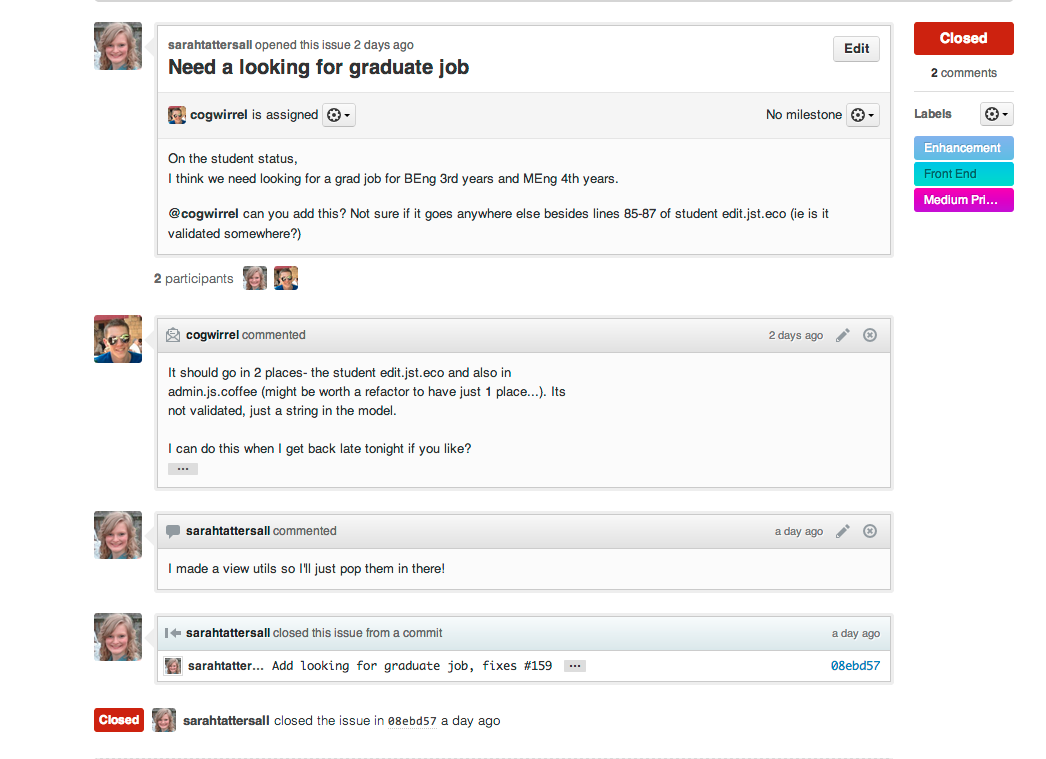
\includegraphics[scale=0.3]{images/project_management/team_management/graduate_issue}
        \caption{Example of a GitHub issue that has been commented on, fixed, and closed}

        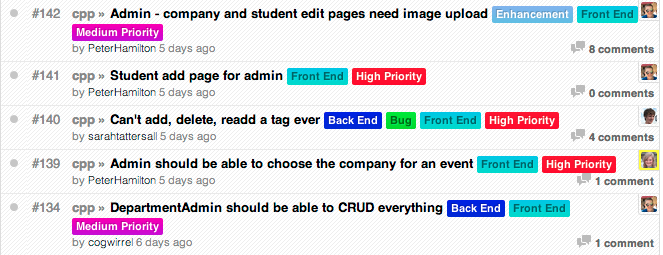
\includegraphics[scale=0.3]{images/project_management/team_management/github_issues}
        \caption{A view of how we see our issue list}
        \end{figure}
        \item \textbf{Pull Requests:} Allow us to show each other changes we've pushed to our repository before merging them into our master branch. We each had a development branch which we would push our requests to and they would then be code reviewed by other members of the team before someone giving the go ahead to `ship it'. Pull requests significantly helped us to spot many bugs before code was pushed into production and to also understand our team members code, giving us a more thorough understanding of the entire code base.
        %TODO PICTURE
        \item \textbf{Automatic backup:} Since our project is backed up with GitHub, we never had to worry about data loss.
    \end{itemize}
    These features have been invaluable for efficient code collaboration.

    \paragraph{Facebook\cite{facebook}} We have also set up a Facebook group including all members to instantly message the entire group, this sustained the collaborative group environment and enabled us to remain in instant contact when working remotely.
    It also stopped Github issues from becoming too chatty.

    \paragraph{CircleCI\cite{circleci}} We used a continuous integration tracker to continuously report on the state of the project, alerting us if the build broke. As we developed we always aimed to maintain the build and found that this encouraged the flow of development as additions where integrated faster into an efficient and stable system advancement.
    We felt that writing weekly reports for the Software Engineering course enabled us to reflect on the group interaction and continuously reminded us to track our progress and apply an Agile development approach.

    \paragraph{Sublime\cite{sublime}} Although, not strictly used for team collaboration we all agreed to use the sublime text editor whilst working on our project. Although sublime has many nice features for development the primary reason we decided to enforce its use is due to the additional package manager\cite{sublime_pm} which enabled the interactive use of git within our text editor.
    The main used feature of this was git commits. When we entered commit mode, we could type out our commit like normal, however under this it shows you the diff of everything you'd changed in the commit. This was handy and aided us in writing descriptive, detailed commits.

    % TODO NEED SOME BETTER RAKE KNOWLEDGE HERE
    \paragraph{rake\cite{rake}} Rake is a Ruby build program and has capabilities similar to make. It allowed us to automate tasks that took many instructions that we performed frequently. One example is when changing an item in the database we would often have to run \verb!rake db:drop; rake db:migrate; rake db:seed; rake db:test:prepare! and to save us from such hassle we created a command \verb!nuke! that did these all for us.

  \subsubsection{Software Design Methodology}
    Throughout our project we followed an Agile software design approach in order to increase group productivity and accelerate code development. We felt that this enabled rapid response to alterations in project requirements and also provided a key factor in ensuring the project progressed according to plan.

    As a group we set milestones to monitor group progress and we ensured that the milestones were met consistently. This was essential in ensuring that the project was delivered on time considering the size and short time-scale of the project. Milestones were set consisting of the requirements outlined in weekly supervisor group meetings. Our Agile approach stimulated group responsiveness to changes in requirements (and new requirements defined in such milestones) by allocating specific tasks for each group member. 

    At a more detailed level within each milestone, we set iterations during frequent group stand up meetings in order to clarify individual member roles and tasks. In order to delegate tasks between the members of the group we divided up the group into Front-end, Back-end and Testing specialist units. Tasks outlined in each iteration would be divided accordingly to the corresponding units and then further assigned to individual group members. We used Trello in the initial stages of the project in order to allocate and divide tasks within iterations to group members, this provided an invaluable project management tool to establish group collaboration and roles. Towards the later stage of the project as group collaboration developed further, and the volume of new tasks decreased, we utilised GitHub issues to outline development issues that needed to be resolved, assigning issues to the specialised group member as they arose from testing and changes to the requirements.

    We felt that GitHub issues were better than a white board of post-it's in a static location because not only does GitHub allow you to access them at any time, anywhere, you can assign different brightly coloured labels to the issues, assign them to a person to complete, comment on the issues and actually see the commits that fixed or broke these issues.

  \subsubsection {Team Member Contributions}
    \paragraph{Pete Hamilton} used his consistent knowledge of Rails and CoffeeScript to aid everyone in their individual challenges. He also up work on some of the more complicated features of our site that required good user understanding of our frameworks to implement.
    \paragraph{Jack Stevenson} worked extensively on client- side development which included the design and implementation of user views, interacting via an API with the server and ...
    \paragraph{Sarah Tattersall} spent most of the early days working on our test suite, she researched the frameworks needed in order to produce DRY (Don't Repeat Yourself) tests and continually researched ways to test new aspects of our site that required extra libraries (such as testing the Views). 
    Whilst implementing tests she also worked on validating the Rails back end models and in the latter half of our project she worked on fixing general GitHub issues that arose, whilst others were working on all the new features we needed.
    \paragraph{Tom Wilding}
    \paragraph{Tom Wilshere}
